%
% File emnlp2016.tex
%

\documentclass[11pt,letterpaper]{article}

\usepackage{emnlp2016}
\usepackage{times}
\usepackage{latexsym}

% \RequirePackage[l2tabu, orthodox]{nag}
% \documentclass{article}

% % FONTS
\usepackage[T1]{fontenc}

% Replace default Latin Modern typewriter with its proportional counterpart
% http://www.tug.dk/FontCatalogue/lmoderntypewriterprop/
\renewcommand*\ttdefault{lmvtt}

\usepackage{amsmath}
\usepackage[subscriptcorrection,
            amssymbols,
            mtpbb,
            mtpcal,
            nofontinfo  % suppresses all warnings
           ]{mtpro2}
\usepackage{scalefnt,letltxmacro}
\LetLtxMacro{\oldtextsc}{\textsc}
\renewcommand{\textsc}[1]{\oldtextsc{\scalefont{1.10}#1}}
\usepackage[scaled=0.92]{PTSans}


% % COLOR
\usepackage[usenames,dvipsnames]{xcolor}
\definecolor{Green}{HTML}{156946}

% % SPACING and TEXT
\usepackage[final,expansion=alltext]{microtype}
\usepackage[english]{babel}
\usepackage{afterpage}
\usepackage{framed}


% define a paragraph header function
\DeclareRobustCommand{\parhead}[1]{\textbf{#1}~}

% % EDITING
% paragraph helper
\DeclareRobustCommand{\PP}{\textcolor{Plum}{\P} }

% % COUNTERS
\renewcommand{\labelenumi}{\color{black!67}{\arabic{enumi}.}}
\renewcommand{\labelenumii}{{\color{black!67}(\alph{enumii})}}
\renewcommand{\labelitemi}{{\color{black!67}\textbullet}}

% FIGURES
\usepackage{graphicx}

% TABLES
\usepackage{booktabs}

% ALGORITHMS
\usepackage[algoruled]{algorithm2e}
\usepackage{listings}
\usepackage{fancyvrb}
\fvset{fontsize=\normalsize}

% % HYPERREF
\usepackage[colorlinks,linktoc=all]{hyperref}
\usepackage[all]{hypcap}
\hypersetup{citecolor=Green}
\hypersetup{linkcolor=Green}
\hypersetup{urlcolor=Green}

% % CLEVEREF must come after HYPERREF
\usepackage[nameinlink]{cleveref}

% BIBLIOGRPHY: get rid of reference labels
\makeatletter
	\renewcommand\@biblabel[1]{}
\makeatother

% ACRONYMS
\usepackage[acronym,smallcaps,nowarn]{glossaries}
% \makeglossaries

% % COLOR DEFINITIONS
\newcommand{\green}[1]{\textcolor{Green}{#1}}


% LISTINGS DEFINTIONS
\lstdefinestyle{mystyle}{
    commentstyle=\color{Green},
    keywordstyle=\color{Green},
    numberstyle=\tiny\color{black!60},
    stringstyle=\color{Green},
    basicstyle=\ttfamily,
    breakatwhitespace=false,
    breaklines=true,
    captionpos=b,
    keepspaces=true,
    numbers=left,
    numbersep=5pt,
    showspaces=false,
    showstringspaces=false,
    showtabs=false,
    tabsize=2
}
\lstset{style=mystyle}

% ALGOZRITHM
\usepackage[algoruled]{algorithm2e}
\DeclareRobustCommand{\mb}[1]{\ensuremath{\boldsymbol{\mathbf{#1}}}}

\DeclareMathOperator*{\argmax}{arg\,max}
\DeclareMathOperator*{\argmin}{arg\,min}

\DeclareRobustCommand{\KL}[2]{\ensuremath{\textrm{KL}\left(#1\;\|\;#2\right)}}

\newcommand{\mbx}{\mathbold{x}}
\newcommand{\mbX}{\mbf{X}}

\newcommand{\mbz}{\mathbold{z}}

\newcommand{\mbI}{\mbf{I}}

\newcommand{\mbZ}{\mbf{Z}}
\newcommand{\mbL}{\mbf{L}}

\newcommand{\mbtheta}{\mathbold{\theta}}
\newcommand{\mbTheta}{\mathbold{\Theta}}
\newcommand{\mbomega}{\mathbold{\omega}}
\newcommand{\mbOmega}{\mathbold{\Omega}}
\newcommand{\mbsigma}{\mathbold{\sigma}}
\newcommand{\mbSigma}{\mathbold{\Sigma}}

\newcommand{\mblambda}{\mathbold{\lambda}}
\newcommand{\mbgamma}{\mathbold{\gamma}}
\newcommand{\mbzeta}{\mathbold{\zeta}}
\newcommand{\mbeta}{\mathbold{\eta}}
\newcommand{\mbbeta}{\mathbold{\beta}}
\newcommand{\mbphi}{\mathbold{\phi}}
\newcommand{\mbmu}{\mathbold{\mu}}
\newcommand{\mbrho}{\mathbold{\rho}}

\newcommand\dif{\mathop{}\!\mathrm{d}}
\newcommand{\diag}{\textrm{diag}}
\newcommand{\supp}{\textrm{supp}}

\newcommand{\E}{\mathbb{E}}
\newcommand{\Var}{\mathbb{V}\textrm{ar}}

\newcommand{\bbN}{\mathbb{N}}
\newcommand{\bbZ}{\mathbb{Z}}
\newcommand{\bbR}{\mathbb{R}}
\newcommand{\bbS}{\mathbb{S}}

\newcommand{\cL}{\mathcal{L}}

\newcommand{\cN}{\mathcal{N}}
\newcommand{\Gam}{\textrm{Gam}}
\newcommand{\InvGam}{\textrm{InvGam}}

\newcommand{\g}{~\vert~}
\newacronym{KL}{kl}{Kullback-Leibler}
\newacronym{ELBO}{elbo}{\emph{evidence lower bound}}
\newacronym{POPELBO}{pop-elbo}{\emph{population evidence lower bound}}

\newacronym{SVI}{svi}{stochastic variational inference}
\newacronym{BUMPVI}{bump-vi}{bumping variational inference}

\newacronym{GMM}{gmm}{Gaussian mixture model}
\newacronym{LDA}{lda}{latent Dirichlet allocation}

\newacronym{SUTVA}{sutva}{stable unit treatment value assumption}

\emnlpfinalcopy
\def\emnlppaperid{116}


\title{Detecting and Characterizing Events}

\author{
Allison J.~B. Chaney\\
    Princeton University\\
	\href{mailto:achaney@cs.princeton.edu}{\nolinkurl{achaney@cs.princeton.edu}}
\And
Hanna Wallach\\
    Microsoft Research\\
    \href{mailto:wallach@microsoft.com}{\nolinkurl{wallach@microsoft.com}}
\AND
Matthew Connelly\\
    Columbia University\\
    \href{mailto:mjc96@columbia.edu}{\nolinkurl{mjc96@columbia.edu}}
\And
David M. Blei\\
    Columbia University\\
    \href{mailto:david.blei@columbia.edu}{\nolinkurl{david.blei@columbia.edu}}
}

\date{}

\begin{document}

\maketitle

\begin{abstract}
%!TEX root = emnlp2016.tex

Significant events are characterized by interactions between entities (e.g., countries, organizations, individuals) that deviate from typical interaction patterns.  Investigators, such as historians, commonly read large quantities of text to construct an accurate picture of who, what, when, and where and event happened.  In this work, we present the Capsule model for analyzing documents to identify and characterize events of potential significance.
Specifically, we develop a model based on topic modeling to distinguish between topics that describe ``business-as-usual'' and topics that deviate from these patterns.
To demonstrate this model, we analyze a corpus of over 2 million US State Department cables from the 1970s; we provide open-source implementations of an inference algorithm for the Capsule model and a pipeline to explore its results.
\end{abstract}



\section{Introduction}
\label{sec:intro}
%!TEX root = submission.tex
% Events are interesting by definition; they are anomalous observations that deviate from the ordinary.  But o


% % Events occur in many sources of data: historical events can be identified from diplomatic messages, scientific events from publications, and network events from communications between users (such as email).  
% % Detecting events automatically is a well-studied problem, but approa

% % We present a model that detects when events occur and characterize.

% % Characterizing an event, however, can prove challenging.  

% \PP why are events interesting?

% \PP what is an event?  (how do we characterize it)

% \PP how can this construction be used? (why do we use the name ``Capsule?'')

% \PP contributions list (vis, model, code for both, exploration on historical corpus and arxiv/enron)

% \PP outline of remainder of paper

% \parhead{Related work.} 

% Automatic event detection is a well-studied problem.  \cite{Neill:2009}

% \PP automatic event detection approaches % see http://www.cs.cmu.edu/~neill/papers/eventdetection.pdf

% \PP topic modeling + viz (incl dynamic topic models)

% \PP network and related work there (e.g. hanna's work); say this isnt explicitly about netorks, but the data has this structure dn the model can be extended to use these concepts (do small experiment where ``entites'' are defined as to/from pairs)




% - anomoly detection, outliers vs events
% - change points
% - social event detection and twitter (incl. locations)
% - event detection in text
% - event summarization in text
% - dynamic topic models and topic modeling viz + hanna's work



\PP event detection is a real-world problem (why interesting?)

\PP what are events?
- they occur rarely
- deviate from normal behavior
- usually affect many datapoints (not just one)
- how does capsule define events?

\PP contibutitions and capsule name

\PP outline of the paper


\parhead{Related work.}  We first review previous work on event detection and other related concepts.  

\PP Automatic event detection is often performed with univariate input data.  In this context, the typical signal is often uniform or a repeating pattern.  Burstiness defiens an event (relate to outliers). poisson processes.  Alternatively, change points. (ordinary changes as you go) 

burtsy: \cite{kleinberg2003bursty}

change points \cite{guralnik1999event} 

\cite{Ihler:2006} univariate data, captures cylical/repreating and rare, persident events (very nice paper), used for prediction
\cite{ihler2007learning} same work?


\cite{weiss1998learning} event prediction (uses genetic algorithm)


%bayseian apprach includes uncertainy and full posterior disyribution

\PP multivariate.  now we can characterize events beyond magnitude.  and work with things like text content.
- Bursty event detection in text: \cite{fung2005parameter} (uses tf-idf, then groups---grouping with topic models first reduces feature space and improves scalability.  this paper has < 100k documents)

\cite{das2008anomaly} anomaly detection is another name for event detection (but not necisarity with time as a dimension).  this paper dies categoriacal data in multi dimensions, but requires trainign dataset (we want unsupervised to just hand it a dataset and learn!)


TEXT:
\cite{mccallum1998comparison} naive bayes classification; teh document is an ``event'' (pbserved events)

\cite{yang2000improving}event tracking; events are manually predetermined

\cite{kumaran2004text} uses tfidf (not scalable), named entities (just another measure for tf-idf, treat them preferentially)


\cite{brants2003system} tfidf

\cite{das2011dynamic} features ; makes distiction between periodic and aperiodic but uses words (not scalable)

\cite{zhao2007temporal} includes rich metadata (sender) for text data 3d: (social, text content, time), content based clustering, again tf-idf (similarity in word space, but then clostered so each document only has one topic...not a mixed membership model)


\cite{pustejovsky2003timeml} int eh complex taxonomy of question-answerign system


\cite{allan1998line} small corpus (even for 1998; cluster into events) 

\cite{li2005probabilistic} news articles and news events; generative model; does event sumarization + basic viz (strange because it's trying to detect events from news articles...each article should already be associated with an event).  


\cite{lau2012line} topic modeling in social media; novel  (essentially find news events from twitter)

\cite{VanDam:2012} each document explicitly recieves a class (topic modeling extension)

\cite{zhang2002novelty} novelty detection (mentions events and first story detecting in news)

\cite{zhao2012novel} bursty text; clusters (efficient, but not really what we want...again using term features)

\cite{wang2007mining} bursty correlated text streams (news events from multiple outlets)

% \PP outliers vs events \cite{Neill:2009} (univariate -> multivariate)
% How is event detection different from:
% 1. SupervisedLearning:
% • Abnormal events are extremely rare, normal events are
% plentiful
% 2. Clustering:
% • Clustering = partitioning data into groups
% • Not the same as finding statistically anomalous groups
% 3. OutlierDetection:
% • Events of interest are usually not individual outliers
% • The event typically affects a subgroup of the data rather than a single data point

summarization:
\cite{peng2007event} events are observations (summarize observtions and dermine relationships between them)
\cite{chakrabarti2011event} events are bursty; collect bursty tweets and summarize them
\cite{gao2012joint} news and tweets toghter; no time series info


\PP other metadata: social netowrks and space (disease breakouts)
social: 
\cite{das2011dynamic} co-bursting; relationship detection between entities (co-mentions)--this is a cpmpletely different problem

\cite{sakaki2010earthquake} user observe real time event; particle filters since twitter is noisy
\cite{jackoway2011identification} breaking news events detected with twitter (includes locations)
\cite{reuter2012event} classify event (scalable) from social media posts
\cite{becker2010learning} identify events and classify (same as above)
\cite{sayyadi2009event} story tracking in social streams

not many of these actually use socialk info...most just use ``social'' just to describe the data source


hanna's paper...\cite{schein2015bayesian} which has sender/reciever adn maps to  (data is counts of labelled interactions at times-a 4 tuple of (sendrr, reciever, acton, time))


spatial: \cite{Neill:2005}
 \cite{mathioudakis2010identifying} identifying and describing spatial bursts
\cite{liu2011using} detect events based on social media activity (incl lat long)



\PP visualizations and interfaces

TODO: \cite{dou2012leadline} uses topic modeling, viualization ** this is main competitor  differences:
 - documents overall (not using author information)
 - deterministic
 - focused on interface and exploration (users can adjust events)




% We first review previous research on event detection, topic modeling, and visualization.

% Automatic event detection is a well-studied problem.  \cite{Neill:2009}




% using social networks to help recommend items to users. A crucial component of SPF is that it infers the influence that users have with each other. In previous work, some systems assume that user influence (sometimes called “trust”) is observed [27]. However, trust information beyond a binary yes/no is onerous for users to input, and thus observing trust beyond “following” or “friending” is impractical in a large system. Others assume that trust is propagated [2] or computed from the structure of the network [10]. This is limited in that it ignores user activity, which can reveal the trust of a user for some parts of the network over others; SPF captures this idea. Information diffusion [8, 12] also relies on user activity to describe influence, but focuses on understanding the widespread flow of information. A final alternative is to compute trust from rating similarities be- tween users [9]. However, performing this computation in advance of fitting the model confounds general preference similarity with instances of influence—two people with the same preferences might read the same books in isolation.

% Other research has included social information directly into vari- ous collaborative filtering methods. Ref. [36] incorporates the net- work into pairwise ranking methods. Their approach is interesting, but one-class ranking methods are not as interpretable as factor- ization, which is important in many applications of recommender systems [15]. Refs. [25, 28, 34] have explored how traditional fac- torization methods can exploit network connections. For example, many of these models factorize both user-item data and the user-user network. This brings the latent preferences of connected users closer to each other, reflecting that friends have similar tastes. Refs [24, 35] incorporate this idea more directly by including friends’ latent representations in computing recommendations made for a user.

% Our model has a fundamentally different approach to using the network to form recommendations. It seeks to find friends with different preferences to help recommend items to a user that are outside of her usual taste. For example, imagine that a user likes an item simply because many of her friends liked it too, but that it falls squarely outside of her usual preferences. Models that adjust
% their friends’ overall preferences according to the social network do not allow the possibility that the user may still enjoy this anomalous item. As we show in Section 3, using the soci



\section{The Capsule Model}
\label{sec:model}
%!TEX root = emnlp2016.tex

In this section we develop the Capsule model.  Capsule captures patterns in entity behavior and identifies events that cause deviations from these patterns among many entities.  The model relies on rich entity behavior data over time, such as messages being sent between entities; text data can summarized (making the model more tractable) with a topic model~\cite{Blei:2012}.  We first review topic models at a high level and give the intuition on Capsule.  Then, we formally specify our model and discuss how we learn the hidden variables.

\parhead{Background: Topic Models.} Capsule relies on topic models to summarize text data, making the model tractable.  Topic models are algorithms for discovering the main themes in a large collection of documents; each document can then be summarized in terms of the global themes.  More formally, a topic $k$ is a probability distribution over the set of vocabulary words.  Each document $d$ is represented as a distribution over topics $\theta_d$.  Thus we can imagine that when we generate a document, we first pick which topics are relevant (and in what proportions); then, for each word, we select a single topic from this distribution over topics, and finally select a vocabulary term from the corresponding topic's distribution over the vocabulary.  We use the LDA topic model~\cite{Blei:2003,Hoffman:2010} to summarize text data, and assume that these summaries are held fixed.  Our model could be extended to include topic modeling as component, but in practice the results would be similar to the stage-wise approach.

\parhead{The Capsule Model.}
Topic models are often applied to provide a structure for an otherwise unstructured collection of documents.  Documents, however, are often accompanied by metadata, such as the date written or author attribution; this information is not exploited by traditional topic models.  The Capsule model uses both author and date information to identify and characterize events that influence the content of the collection.

Consider an entity like the Bangkok American embassy, shown in Figure~\ref{fig:cartoon}.  We can imagine that there is a stream of messages (or \emph{diplomatic cables}) being sent by this embassy---some might be sent to the US State Department, others to another American embassy like Hong Kong.  An entity will usually talk about certain topics; the Bangkok embassy, for instance, is concerned with topics regarding southeast Asia more generally.

Now imagine that at a particular time, an event occurs, such as the capture of Saigon during the Vietnam war.  We do not directly observe that events occur, but each event can again be described in the same topic space used to describe individual messages.  Further, when an event occurs, the message content changes for multiple entities. The day following the capture of Saigon, the majority of the diplomatic cables sent by the Bangkok embassy were about Vietnam war refugees.
Thus we imagine that an entity's stream of messages is controlled by what it usually talks about as well as the higher level stream of unobserved events.

\parhead{Model Specification.}
% We formally describe Capsule. The observed data are documents represented in topic space; each document has an author (or entity) and a time (or date) associated with it.  The document content for each document $d$ is represented as $\theta_d$, a $K$-dimensional vector, where $K$ is the number of topics.  The author and time associated with document $d$ are represented as $n_d$ and $m_d$, respectively.

% The hidden variables of this model are the authors' typical concerns, event occurrences, and event descriptions.  We represent the concerns of author $n$ as $\phi_n$, also a $K$-dimensional topic vector.  For each time $t$ we represent whether or not an event occurs with $\epsilon_t$; when an event does occur we represent its content as $\pi_t$, another $K$-dimensional topic vector.

% Conditional on the hidden variables and the author and time metadata, Capsule is a model of how document topics $\theta_d$ came to be; we generate the topics for each document
% \begin{equation}
% \theta_{d,k} \sim \mbox{Gamma}\left(\phi_{n_d,k} + \sum_{t=1}^T f(t, m_d) \epsilon_t \pi_{t,k}\right),\footnotemark
% \end{equation}
% % \footnotetext{Throughout this work, we use a non-traditional parameterization of the gamma distribution.  Recall the shape $a$ and scale $b$ parameterization of the gamma, or \[\mbox{Gamma}^*(x \g a, b) = \frac{1}{\Gamma(a) b^a} x^{(a-1)}e^{- x / b}.\] In our alternative parameterization, we use a single mean parameter $\mu$ and a fixed sparsity hyperparameter $\alpha$, or \[\mbox{Gamma}(x \g \mu, \alpha) = \mbox{Gamma}^*(x \g \alpha, \mu / \alpha);\] when a gamma distribution is only specified by a single parameter, it is the mean $\mu$ and the sparsity hyperparamter $\alpha$ is hidden for simplicity.
% % }
% where we define the event decay function $f$ to be a simple linear decrease: \[f(t, m) =
% \begin{cases}
%   1 - \frac{m-t}{\delta}, & \mbox{if } t \le m < t+\delta \\
%   0, & \mbox{otherwise,}
% \end{cases} \] with $\delta$ being the time duration after the event at time $t$ is no longer relevant.  Figure~\ref{fig:graphicalmodel} shows the dependencies between the hidden and observed variables as a graphical model.

% To complete the specification of all the variables, we place priors on all of the hidden variables.  Author concerns $\phi_{n,k}$ and event content $\pi_t$ are specified with Gamma priors.  Event occurrence $\epsilon_t$ has a Poisson prior.
% % TODO: we make a note about the Poisson taking values > 1; what is the intuition?

% \begin{figure}
% \centering
% 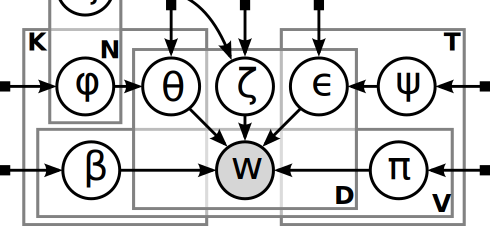
\includegraphics[width=0.5\linewidth]{fig/graphicalmodel.pdf}
% \caption{A directed graphical model of Capsule to show considered dependencies. Shaded document topics nodes $\theta$ are observed. unshaded nodes are hidden variables---these are event occurrences $\epsilon$, event content descriptions $\pi$, and entity typical concerns $\phi$. Plates denote replication: there are $D$ documents, $T$ time steps, $N$ entities, and $K$ topics. Hyperparameters $\eta$, $\mu$, and $\alpha$ are fixed.}
% \label{fig:graphicalmodel}
% \end{figure}

\begin{figure}
\begin{mdframed}
\small
\begin{itemize}[leftmargin=*]
\item for each time step $t=$~1:$T$,
	\begin{itemize}[leftmargin=*]
	\item draw event description over vocabulary \\$\pi_t \sim \mbox{Dirichlet}_V (\alpha)$
	\item draw event strength \\$\psi_{t} \sim \mbox{Gamma}(s_\psi, r_\psi)$
	\end{itemize}
\item for each topic $k=$~1:$K$,
	\begin{itemize}[leftmargin=*]
	\item draw topic distribution over vocabulary \\$\beta_k \sim \mbox{Dirichlet}_V (\alpha)$
	\item for each entity $n=$~1:$N$,
		\begin{itemize}[leftmargin=*]
		\item draw entity concern \\$\phi_{n,k} \sim \mbox{Gamma}(s_\phi, r_\phi)$
		\end{itemize}
	\end{itemize}
\item for each document $d=$~1:$D$ sent at time $i_d$ by author $a_d$,
	\begin{itemize}[leftmargin=*]
		\item for each topic $k=$~1:$K$,
		\begin{itemize}[leftmargin=*]
			\item draw local entity concern \\$\theta_{d,k} \sim \mbox{Gamma}(s_\theta, \phi_{a_d,k})$
		\end{itemize}
	\item for each time $t=$~1:$T$,
		\begin{itemize}[leftmargin=*]
			\item draw local event relevancy \\$\epsilon_{d,t} \sim \mbox{Gamma}(s_\epsilon, \psi_{i_d,t})$ 
		\end{itemize}
	\item for each vocabulary term $v=$~1:$V$,
		\begin{itemize}[leftmargin=*]
			\item draw word counts $w_{d,v} \sim\\ \mbox{Poisson}\left(\theta_d^\top\beta_v + \sum_{t=1}^T f(i_d, t) \epsilon_{d,t} \pi_{t,v}\right)$
		\end{itemize}
	\end{itemize}
\end{itemize}
\end{mdframed}
\caption{The generative process for Capsule.}
\label{fig:generative-model}
\end{figure}


\parhead{Learning the hidden variables.}
In order to use the Capsule model to explore the observed documents, we must compute the posterior distribution.  Conditional on the observed word counts $w$, our goals to to compute the posterior values of the hidden parameters---global event strengths $\psi$, event descriptions $\pi$, entity concerns $\phi$, and topics $\beta$, as well as document-specific entity concerns $\theta$ and event relevancy parameters $\epsilon$.

As for many Bayesian models, the exact posterior for Capsule is not tractable to compute; approximating it is our central statistical and computational problem.  We develop an approximate inference algorithm for Capsule based on variational methods~\cite{Wainwright:2008}.\footnote{Source code is available at https://github.com/?????/capsule.}

Variational inference approaches the problem of posterior inference by minimizing the KL divergence from an approximating distribution $q$ to the true posterior $p$.
This is equivalent to maximizing the ELBO,
\begin{multline}
	\mathcal{L}(q)  = \E_{q(\psi, \pi, \phi, \beta, \theta, \epsilon)}\bigl[\log p(w, \psi, \pi, \phi, \beta, \theta, \epsilon) \\
	-~\log q(\psi, \pi, \phi, \beta, \theta, \epsilon)\bigr].
	\label{eq:elbo}
\end{multline}

We define the approximating distribution $q$ using the mean field assumption:
\begin{multline}
	q(\psi, \pi, \phi, \beta, \theta, \epsilon) = \prod_{t=1}^T \left[ q(\pi_{t} \g \lambda^\pi_t) q(\psi_t \g \lambda^\psi_t) \right] \\
		\prod_{k=1}^K \left[ q(\beta_{k} \g \lambda^\beta_k) \prod_{n=1}^N q(\phi_{n,k} \g \lambda^\phi_{n,k}) \right] \\
		\prod_{d=1}^D \left[
				\prod_{k=1}^K q(\theta_{d,k} \g \lambda^\theta_{d,k})
				\prod_{t=1}^T q(\epsilon_{d,t} \g \lambda^\epsilon_{d,t})
			\right]
	\label{eq:q}
\end{multline}

The variational distributions $q(\pi)$ and $q(\beta)$ are both Dirichlet-distributed with free variational parameters $\lambda^\pi$ and $\lambda^\beta$, respectively.  Similarly, $q(\psi)$, $q(\phi)$, $q(\theta)$ and $q(\epsilon)$ are all gamma-distributed with corresponding free variational parameters $\lambda^\psi$, $\lambda^\phi$, $\lambda^\theta$, and $\lambda^\epsilon$.

The expectations under $q$, which are needed to maximize the ELBO, have closed form analytic updates, as detailed in Appendix~\ref{sec:inference}. We update each parameter in turn, following standard coordinate ascent variational inference techniques.  Full details on our inference algorithm can be found in the appendix.  This algorithm produces a fitted variational distribution which can then be used as a proxy for the true posterior, allowing us to explore a collection of documents with Capsule.  

\parhead{Visualization.}
Capsule is a high-level statistical tool. In order to understand and explore its results, a user must scrutinize numerical distributions.
To make Capsule more accessible, we developed an open source tool for visualizing its results.\footnote{Source code: https://github.com/?????/capsule-viz.}  Our tool creates a navigator of the documents and latent parameters, allowing users to explore events, entities, topics, and the original documents.  Figure~\ref{fig:viz} shows several screenshots of this browsing interface.

\begin{figure}
\centering
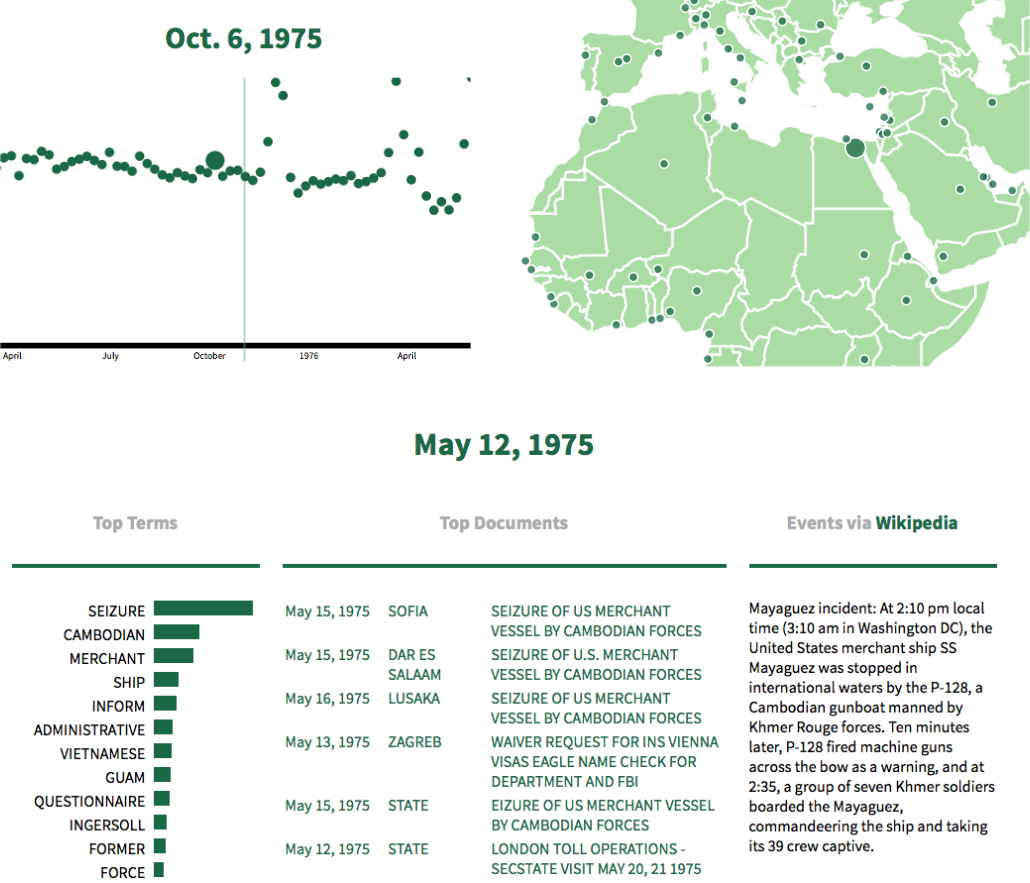
\includegraphics[width=\linewidth]{fig/viz.png}
\caption{Screenshots of Capsule visualization of US State Department cables.  Left: top words in a topic (manually labeled topic title).  Center-top: events over time (height is volume of messages sent, color is probability of an event occurring).  Center-bottom: topics for an event on <date TODO: cyprus coup?>.  Right-top: cyprus entity topics? TODO.  Right-bottom: entities shown on a map.}
\label{fig:viz}
\end{figure}


%\section{Evaluation}
%\label{sec:eval}
\PP outline two datasets (cables and enron) and the tasks to be done

\subsection{Data}
\parhead{Cables}

\parhead{arXiv}

\parhead{Enron}


\PP insert table and refetence for both (number of days, entities, total messages, or something); maybe a plot showing attributes of the data...somehow inform them that the state department is a bias for the cables data

\PP footnote on handling multiple recipients of message...

\subsection{Metrics and competing methods}

\PP how we evaluate based on real events

\PP how we evaluate based on perplexity (prediction of words)

\PP competing methods for perplexity: LDA, average user words?, dynamic topic model, network topic models

\subsection{Performance and exploration}

\PP sumry of comparison to gold-standard events for cables

\PP table of predictive likelihood results and summary pgh; and/or cite tea leaves paper

\parhead{Exploration}

\PP charachetrize events manually (based on cables) vs event detection characterization

\PP show descriptions for cables entities and select events; same for arxiv/enron

\PP any other exploration you can think of!


Results: ROC curve (x=false postive rate, y=true postive rate)

\section{Conclusion}
\label{sec:discussion}
%!TEX root = emnlp2016.tex

We presented Capsule, a Bayesian model for detecting and
characterizing potentially significant events. We evaluated Capsule's
ability to detect events and find relevant messages; it outperformed four 
baseline methods. We used Capsule to analyze a large corpus of U.S. State 
Department cables from the 1970s, demonstrating 
that it can discover both well-known and obscure (but 
significant) events, as well as relevant documents;
this is increasingly important---it
is estimated that the State Department 
produces two billion e-mails annually. 
We anticipate that Capsule, and our
visualization tool, will be useful for historians, political
scientists, and journalists who wish to explore and understand large
corpora of documents.



% \small
\section*{Acknowledgments}
This work was supported by NSF IIS-1247664; ONR N00014-11-1-0651;
DARPA FA8750-14-2-0009 and N66001-15-C-4032; Adobe; the Alfred
P. Sloan Foundation; the Columbia Global Policy Initiative.

\onecolumn
\vspace*{20px}
\section*{\Large\centering Appendices}
\vspace{50px}

\appendix
\section{Inference}
% REMINDER: comment out page break temporarily to compile!
\label{sec:inference}
%!TEX root = supplemental.tex

In this appendix, we describe the details of the inference algorithm for Capsule.

Conditional on a collection of observed documents, our goal is to estimate the posterior values of the hidden parameters, according to the Capsule model.   Recall that our data is observed as word counts $n_{dv}$ for document $d$ and vocabulary term $v$, with corresponding author and time interval information for each document---$a_d$ and $t_d$, respectively.
The latent parameters of the model include general topics $\mathbold{\beta}_1, \ldots, \mathbold{\beta}_K$, entity topics $\mathbold{\eta}_1, \ldots, \mathbold{\eta}_A$, and event topics $\mathbold{\gamma}_1, \ldots, \mathbold{\gamma}_T$, as well as message-specific strengths in each of these spaces: document relevancy to general topics $\mathbold{\theta}_d$, entity topics $\zeta_d$, and interval topics $\mathbold{\epsilon}_d$.  The latent parameters also include entity concerns with general topics $\mathbold{\phi}_1, \ldots, \mathbold{\phi}_A$ and with entity-specific topics $\xi_1, \ldots, \xi_A$, and overall event strength $\psi_1, \ldots, \psi_T$.  See \Cref{fig:generative-model} for the full generative model.

As for many Bayesian models, the exact posterior for Capsule is not tractable to compute; we must instead approximate it.  Thus, we develop an approximate inference algorithm for Capsule based on variational methods~\cite{Jordan:1999,Wainwright:2008}.

Variational inference approaches the problem of posterior inference by minimizing the KL divergence from an approximating distribution $q$ to the true posterior $p$.
This is equivalent to maximizing the ELBO,
\begin{equation}
	\mathcal{L}(q)  = \E_{q}\bigl[\log p(\mathbf{W}, \mathbold{\psi}, \mathbold{\gamma}, \mathbold{\phi}, \mathbold{\beta}, \mathbold{\xi}, \mathbold{\eta}, \mathbold{\theta}, \mathbold{\epsilon}, \mathbold{\zeta})
	- \log q(\mathbold{\psi}, \mathbold{\gamma}, \mathbold{\phi}, \mathbold{\beta}, \mathbold{\xi}, \mathbold{\eta}, \mathbold{\theta}, \mathbold{\epsilon}, \mathbold{\zeta})\bigr].
	\label{eq:cables:elbo}
\end{equation}


We define the approximating distribution $q$ using the mean field assumption:
\begin{multline}
	q(\mathbold{\psi}, \mathbold{\gamma}, \mathbold{\phi}, \mathbold{\beta}, \mathbold{\xi}, \mathbold{\eta}, \mathbold{\theta}, \mathbold{\epsilon}, \mathbold{\zeta}) = 
	 	\prod_{d=1}^D \left[q(\zeta_d \g \lambda_d)
				\prod_{k=1}^K q(\theta_{dk} \g \lambda^\theta_{dk})
				\prod_{t=1}^T q(\epsilon_{dt} \g \lambda^\epsilon_{dt})
			\right] \\
		\prod_{t=1}^T \left[ q(\mathbold{\gamma}_{t} \g \lambda^\gamma_t) q(\psi_t \g \lambda^\psi_t) \right] 
		\prod_{a=1}^A \left[ q(\xi_{a} \g \lambda^\xi_{a})~q(\mathbold{\eta}_a \g \lambda^{\eta}_{a}) \right] 
		\prod_{k=1}^K \left[ q(\mathbold{\beta}_{k} \g \lambda^\beta_k) \prod_{a=1}^A q(\phi_{ak} \g \lambda^\phi_{ak}) \right]
	\label{eq:q}
\end{multline}

The variational distributions for the topics $q(\mathbold{\gamma}_t)$, $q(\mathbold{\beta}_k)$ and $q(\mathbold{\eta}_a)$ are all Dirichlet-distributed with free variational parameters $\lambda^\gamma$, $\lambda^\beta$, and $\lambda^\eta$ respectively.  Similarly, the variational distributions $q(\psi_t)$, $q(\phi_{ak})$, $q(\xi_a)$, $q(\theta_{dk})$, $q(\epsilon_{dt})$, and $q(\zeta_d)$ are all gamma-distributed with corresponding free variational parameters $\lambda^\psi$, $\lambda^\phi$, $\lambda^\xi$, $\lambda^\theta$, $\lambda^\epsilon$ and $\lambda^\zeta$.  For these gamma-distributed variables, each free parameter $\lambda$ has two components: shape $s$ and rate $r$.

The expectations under $q$, which are needed to maximize the ELBO, have closed form analytic updates--we update each parameter in turn, following standard coordinate ascent variational inference techniques, as the Capsule model is specified with the required conjugate relationships that make this approach possible~\cite{Ghahramani:2001}.


To obtain simple updates, we first rely on auxiliary latent variables $z$. These variables, when marginalized out, leave the original model intact. The Poisson distribution has an additive property; specifically if $w \sim \mbox{Poisson}(a+b)$, then $w = z_1 + z_2$, where $z_1 \sim \mbox{Poisson}(z_1)$ and $z_2 \sim \mbox{Poisson}(z_2)$.  We apply this property to the word count rate in \Cref{eq:poisrate} and define Poisson variables for each component of the word count:
\[ z^\mathcal{K}_{dvk} \sim \mbox{Poisson}(\theta_{dk}\beta_{kv}), \]
\[ z^\mathcal{A}_{dv} \sim \mbox{Poisson}(\zeta_{d}\eta_{a_dv}), \]
\[ z^\mathcal{T}_{dvt} \sim \mbox{Poisson}\left(f(t_d, t) \epsilon_{dt} \gamma_{tv}\right). \]
The $\mathcal{K}$, $\mathcal{A}$, and $\mathcal{T}$ superscripts indicate the contributions from general, entity, and event topics, respectively.  Given these variables, the total word count is deterministic:
\[ n_{dv} = \sum_{k=1}^K z^\mathcal{K}_{dvk} + z^\mathcal{A}_{d} + \sum_{t=1}^T z^\mathcal{T}_{dvt}. \]

Coordinate-ascent variational inference is derived from complete conditionals, i.e., the conditional distributions of each variable given the other variables and observations. These conditionals define both the form of each variational factor and their updates. The following are the complete conditional for each of the gamma- and Dirchlet-distributed latent parameters.  The notation $D(n)$ is used for the set of documents sent by entity $n$; $D(t)$ is the set of documents sent impacted by events at time $t$ (e.g., all documents after the event in the case of exponential decay).
\begin{equation}
\mathbold{\gamma}_t \g \mathbf{N}, \mathbold{\psi}, \mathbold{\phi}, \mathbold{\beta}, \mathbold{\xi}, \mathbold{\eta}, \mathbold{\theta}, \mathbold{\epsilon}, \mathbold{\zeta}, \mathbf{z} \sim 
	\mbox{Dirichlet}_V\left(\alpha + \sum_{d=1}^D
		z^\mathcal{T}_{d1t}, \dots, \alpha + \sum_{d=1}^D z^\mathcal{T}_{dVt}
	\right)
\label{eq:pi}
\end{equation}
\begin{equation}
\mathbold{\eta}_n \g \mathbf{N}, \mathbold{\psi}, \mathbold{\gamma}, \mathbold{\phi}, \mathbold{\beta}, \mathbold{\xi}, \mathbold{\theta}, \mathbold{\epsilon}, \mathbold{\zeta}, \mathbf{z} \sim 
	\mbox{Dirichlet}_V\left(\alpha + \sum_{d\in D(n)}
		z^\mathcal{A}_{dv}, \dots, \alpha + \sum_{d\in D(n)} z^\mathcal{A}_{dv}
	\right)
\label{eq:eta}
\end{equation}
\begin{equation}
\mathbold{\beta}_k \g \mathbf{N}, \mathbold{\psi}, \mathbold{\gamma}, \mathbold{\phi}, \mathbold{\xi}, \mathbold{\eta}, \mathbold{\theta}, \mathbold{\epsilon}, \mathbold{\zeta}, \mathbf{z} \sim
	\mbox{Dirichlet}_V\left(\alpha + \sum_{d=1}^D
		z^\mathcal{K}_{d1k}, \dots, \alpha + \sum_{d=1}^D z^\mathcal{K}_{dVk}
	\right)
\label{eq:beta}
\end{equation}
\begin{equation}
\psi_t \g \mathbf{N}, \mathbold{\gamma}, \mathbold{\phi}, \mathbold{\beta}, \mathbold{\xi}, \mathbold{\eta}, \mathbold{\theta}, \mathbold{\epsilon}, \mathbold{\zeta}, \mathbf{z} \sim 
	\mbox{Gamma}\left(
		s + |D(t)| s,
		r + \sum_{d\in D(t)} \epsilon_{dt}
	\right)
\label{eq:psi}
\end{equation}
\begin{equation}
\xi_n \g \mathbf{N}, \mathbold{\psi}, \mathbold{\gamma}, \mathbold{\phi}, \mathbold{\beta}, \mathbold{\eta}, \mathbold{\theta}, \mathbold{\epsilon}, \mathbold{\zeta}, \mathbf{z} \sim 
	\mbox{Gamma}\left(
		s + |D(n)| s,
		r + \sum_{d\in D(n)} \zeta_{d}
	\right)
\label{eq:xi}
\end{equation}
\begin{equation}
\phi_{nk} \g \mathbf{N}, \mathbold{\psi}, \mathbold{\gamma}, \mathbold{\beta}, \mathbold{\xi}, \mathbold{\eta}, \mathbold{\theta}, \mathbold{\epsilon}, \mathbold{\zeta}, \mathbf{z} \sim 
	\mbox{Gamma}\left(
		s + |D(n)| s,
		r + \sum_{d\in D(n)} \theta_{dk}
	\right)
\label{eq:phi}
\end{equation}
\begin{equation}
\theta_{dk} \g \mathbf{N}, \mathbold{\psi}, \mathbold{\gamma}, \mathbold{\phi}, \mathbold{\beta}, \mathbold{\xi}, \mathbold{\eta}, \mathbold{\epsilon}, \mathbold{\zeta}, \mathbf{z} \sim 
	\mbox{Gamma}\left(
		s + \sum_{v=1}^V z^\mathcal{K}_{dvk},
		\phi_{a_d k} + \sum_{v=1}^V \beta_{kv}
	\right)
\label{eq:theta}
\end{equation}
\begin{equation}
\epsilon_{dt} \g \mathbf{N}, \mathbold{\psi}, \mathbold{\gamma}, \mathbold{\phi}, \mathbold{\beta}, \mathbold{\xi}, \mathbold{\eta}, \mathbold{\theta}, \mathbold{\zeta}, \mathbf{z} \sim 
	\mbox{Gamma}\left(
		s + \sum_{v=1}^V z^\mathcal{T}_{dvt},
		\psi_t + f(t_d, t) \sum_{v=1}^V \gamma_{tv}
	\right)
\label{eq:epsilon}
\end{equation}
\begin{equation}
\zeta_{d} \g \mathbold{\psi}, \mathbold{\gamma}, \mathbold{\phi}, \mathbold{\beta}, \mathbold{\xi}, \mathbold{\eta}, \mathbold{\theta}, \mathbold{\epsilon}, \mathbf{z} \sim 
	\mbox{Gamma}\left(
		s + \sum_{v=1}^V z^\mathcal{A}_{dv},
		\xi_{a_d} + \sum_{v=1}^V \eta_{a_d v}
	\right)
\label{eq:zeta}
\end{equation}

The complete conditional for the auxiliary variables has the form
\[\mathbf{z}_{dv} \g \mathbf{N}, \mathbold{\psi}, \mathbold{\gamma}, \mathbold{\phi}, \mathbold{\beta}, \mathbold{\xi}, \mathbold{\eta}, \mathbold{\theta}, \mathbold{\epsilon}, \mathbold{\zeta} \sim \mbox{Mult}(n_{dv}, \mathbold{\omega}_{dv}),\] where
\begin{equation}
\mathbold{\omega}_{dv} \propto \langle 
\theta_{d1} \beta_{1v}, \dots, \theta_{dK} \beta_{Kv}, \zeta_d \eta_{a_d v}, 
f(t_d, 1) \epsilon_{d1} \gamma_{1v}, \dots, f(t_d, T) \epsilon_{dT} \gamma_{Tv}\rangle.
\label{eq:omega}
\end{equation}
Intuitively, these variables allocate the data to one of the entity concerns or events, and thus can be used to explore the data.

Given these conditionals, the algorithm sets each parameter to the expected conditional parameter under the variational distribution. The mean field assumption guarantees that this expectation will not involve the parameter being updated.  \Cref{alg:capsule} shows our variational inference algorithm.

This algorithm uses the notation $\mathbold{\lambda}$ to refer to the set of variational parameters,
\[\mathbold{\lambda} = \{\lambda^\gamma, \lambda^\eta, \lambda^\beta, \lambda^\psi, \lambda^\zeta, \lambda^\phi, \lambda^\theta, \lambda^\epsilon, \lambda^\xi\}.\] The notation $V(d)$ is the set of vocabulary indices for the collection of words in document $d$.  We could also iterate over all $V$, but as zero word counts give $\E[\mathbf{z}_{dv}] = 0~\forall v \not\in V(d)$, the two are equivalent.

%TODO: check for consistent indexing of variables (e.g., beta_{v,k} vs beta_{k,v})


\begin{algorithm}[p]
\small
\DontPrintSemicolon
\KwIn{word counts $w$}
%($\psi$, $\gamma$, $\xi$, $\eta$, $\phi$, $\beta$, $\theta$, $\zeta$, $\epsilon$)
\KwOut{approximate posterior of latent parameters in terms of variational parameters $\mathbold{\lambda}$}
\textbf{Initialize} $\E[\mathbold{\beta}_k]$ to slightly random around uniform for each $k$\;
\textbf{Initialize} $\E[\mbox{all other parameters}]$ to uniform \;
\For {iteration $m=1, dots, M$}{
	\textbf{set} all $\mathbold{\lambda}$ to respective priors, excluding $\lambda^{\theta,rate}$, $\lambda^{\zeta,rate}$, and $\lambda^{\epsilon,rate}$, which are set to 0 \;
	\textbf{update} $\lambda^{\theta,rate}_{dk} \pluseq \sum_V \E[\mathbold{\beta}_{kv}]$  for all messages $d$ and topics $k$\;
	\For {each message $d=1, \dots, D$}{
		\For {each term $v\in V(d)$\footnotemark}{
			\textbf{set} $(K+T+1)$-vector $\mathbold{\omega}_{dv}$ as shown in \cref{eq:omega}, using $\E$ of parameters\;
			\textbf{set} $(K+T)$-vector $\E[\mathbf{z}_{dv}] = n_{dv} * \mathbold{\omega}_{dv}$ \;
			\textbf{update} $\lambda^{\theta,shape}_{dk} \pluseq \E[z^\mathcal{K}_{dvk}]$ for all $k$ [\cref{eq:theta}]\;
			\textbf{update} $\lambda^{\epsilon,shape}_{dt} \pluseq \E[z^\mathcal{K}_{dvt}]$ for all $t$ [\cref{eq:epsilon}]\;
			\textbf{update} $\lambda^{\zeta,shape}_d \pluseq \E[z^\mathcal{A}_{dv}]$ [\cref{eq:zeta}]\;

			\textbf{update} $\lambda^{\beta}_{kv} \pluseq \E[z^\mathcal{K}_{dvk}]$ for all $k$ [\cref{eq:beta}]\;
			\textbf{update} $\lambda^{\gamma}_{tv} \pluseq \E[z^\mathcal{T}_{dvt}]$ for all $t$ [\cref{eq:pi}]\;
			\textbf{update} $\lambda^{\eta}_{a_d v} \pluseq \E[z^\mathcal{A}_{dv}]$ [\cref{eq:eta}]\;
		}

		\textbf{set} $\lambda^{\theta,rate}_{dk} = \E[\phi_{a_d k}] +\sum_v \E[\beta_{kv}]$ for all $k$ [\cref{eq:theta}]\;
		\textbf{set} $\lambda^{\epsilon,rate}_{dt} = \E[\psi_t] + f\sum_v \E[\gamma_{tv}]$ for all $t$ [\cref{eq:epsilon}]\;
		\textbf{set} $\lambda^{\zeta,rate}_{d} = \E[\xi_{a_d}] + \sum_v\E[\eta_{a_d v}]$ [\cref{eq:zeta}]\;
		
		\textbf{set} $\E[\theta_{dk}] = \lambda^{\theta,shape}_{dk} / \lambda^{\theta,rate}_{dk}$ for all $k$\;
		\textbf{set} $\E[\epsilon_{dt}] = \lambda^{\epsilon,shape}_{dt} / \lambda^{\epsilon,rate}_{dt}$ for all $t$\;
		\textbf{set} $\E[\zeta_d] = \lambda^{\zeta,shape}_d / \lambda^{\zeta,rate}_d$ \;
		
		\textbf{update} $\lambda^{\phi,shape}_{a_d k} \pluseq s$ for all $k$ [\cref{eq:phi}] \;
		\textbf{update} $\lambda^{\psi,shape}_{t} \pluseq s \forall t : f(t_d, t) \neq 0$ [\cref{eq:psi}] \;
		\textbf{update} $\lambda^{\xi,shape}_{a_d} \pluseq s$ [\cref{eq:xi}] \;
		\textbf{update} $\lambda^{\phi,rate}_{a_d k} \pluseq \theta_{dk}$ for all $k$ [\cref{eq:phi}] \;
		\textbf{update} $\lambda^{\psi,rate}_t \pluseq \epsilon_{dt}$ for all $t$ [\cref{eq:psi}] \;
		\textbf{update} $\lambda^{\xi,rate}_{a_d} \pluseq \zeta_d$ [\cref{eq:xi}] \;

	}

	\textbf{set} $\E[\phi_{ak}] = \lambda^{\phi,shape}_{ak} / \lambda^{\phi,rate}_{ak}$ for all $a$ and $k$ \;
	\textbf{set} $\E[\mathbold{\beta}_{k}] = \mathbold{\lambda}^{\beta}_{k} / \sum_v \lambda^{\beta}_{kv}$ for all $k$ \;
	\textbf{set} $\E[\xi_{d}] = \lambda^{\xi,shape}_d / \lambda^{\xi,rate}_d$ for all $d$ \;
	\textbf{set} $\E[\mathbold{\eta}_{a}] = \mathbold{\lambda}^{\eta}_{a} / \sum_v \lambda^{\eta}_{nv}$ for all $a$ \;
	\textbf{set} $\E[\psi_a] = \lambda^{\psi,shape}_a / \lambda^{\psi,rate}_a$ for all $a$\;
	\textbf{set} $\E[\mathbold{\gamma}_t] = \mathbold{\lambda}^{\gamma}_t / \sum_v \lambda^{\gamma}_{tv}$ for all $t$ \;
}
\Return{$\mathbold{\lambda}$} \;
\caption{Variational Inference for Capsule}
\label{alg:capsule}
\end{algorithm}

This algorithm produces a fitted variational distribution which can then be used as a proxy for the true posterior, allowing us to explore a collection of documents with Capsule.  Source code is available at \url{https://github.com/ajbc/capsule}.




\section{Additional Results}
\label{sec:additional_results}
%!TEX root = supplemental.tex

In this appendix, we provide additional results for
 Capsule. \Cref{tab:entebbe} lists the highest-ranked messages for an
 event described in \cref{sec:eval}. \Cref{tab:topics,tab:entities}
 contain examples of general topics and entity topics, respectively.

\begin{table*}[htb]
\small
\centering
\begin{tabular}{cccc}
\toprule
$f(t_d, t)\,\E[\epsilon_{dt}]$ & \textbf{Date} & \textbf{Author Entity} & \textbf{Subject} \\
\midrule
6.86 & 1976-07-07 & Cairo & Possible SC meeting on Israeli rescue operation \\
6.18 & 1976-07-10 & Kuwait & Media reaction to Bicentennial summary \\
6.15 & 1976-07-06 & Damascus & Syria condemns Israeli operation to free Air France ... \\
5.91 & 1976-07-08 & Tel Aviv & Passengers comment on Air France hijacking \\
5.89 & 1976-07-06 & Stockholm & Possible SC meeting on Israeli rescue operation \\
5.38 & 1976-07-09 & Nicosia & Bicentennial activities in Cyprus \\
5.09 & 1976-07-11 & State & Security Council debate on Entebbe events CONFID... \\
4.77 & 1976-07-09 & State & Travel of Peter M.~Storm, House Budget Committee \\
4.76 & 1976-07-06 & Jidda & Weekly Saudi Editorial Summary (June 30-July 6) \\
4.68 & 1976-07-08 & Lusaka & SWAPO President seeks assessment of Kissinger-Vor... \\
4.56 & 1976-07-07 & Stockholm & Ugandan role in Air France hijacking \\
4.45 & 1976-07-06 & Karachi & Transitional quarter funding for RSS travel \\
4.43 & 1976-07-06 & Athens & Bicentennial anniversary in Greece \\
4.37 & 1976-07-08 & Damascus & Beirut travel \\
4.34 & 1976-07-10 & State & Status of Mrs. Bloch \\
4.17 & 1976-07-07 & Hong Kong & Hong Kong Communist press denounces Israeli resc... \\
4.12 & 1976-07-08 & Dar es Salaam & President Nyerere's fourth of July messages \\
4.09 & 1976-07-10 & Moscow & Pravda and Krasnaya Zvezda on Entebbe rescue oper... \\
\bottomrule
\end{tabular}
\caption{Highest-ranked messages for the week immediately following the U.S.
Bicentennial Celebration and Operation Entebbe. Capsule accurately
recovers messages related to both of these real-world events. Typos
are intentionally copied from the data.}
\label{tab:entebbe}
\end{table*}

\begin{table*}[htb]
\centering
\small
\begin{tabular}{c}
\toprule
\textbf{Top Terms} \\
\midrule
church, vatican, catholic, bishop, pope, ford, cardinal, ban, religious, archbishop \\
program, university, grant, education, school, post, institute, research, center, american \\
security, council, terrorist, threat, sc, sabotage, protective, herein, unsc, honour \\
visit, hotel, schedule, arrival, arrive, depart, please, meet, day, room \\
labor, union, strike, ilo, employment, federation, afl cio, trade, worker, confederation \\
bank, credit, loan, investment, finance, payment, financial, eximbank, opic, central \\
law, case, court, legal, investigation, arrest, justice, sentence, trial, attorney \\
party, government, election, opposition, national, leader, campaign, vote, support, anti \\
tax, company, pay, lease, compensation, exemption, repatriation, income, taxation, fee \\
oil, petroleum, opec, crude, gulf, price, exploration, refinery, energy, company \\
israel, arab, israeli, middle, egypt, peace, plo, cairo, egyptian, lebanon \\
radio, television, broadcast, allotment, appropriation, obligation, zero, warc, transmitter, network \\
india, indian, pakistan, delhi, goi, ocean, bangladesh, transit, pakistani, afghan \\
turkish, turkey, cyprus, greek, greece, athens, ankara, morocco, cypriot, algeria \\
aid, relief, emergency, usaid, disaster, donor, wfp, sahel, ifad, unicef \\
aircraft, team, flight, clearance, transport, civair, aviation, traffic, charter, cargo \\
soviet, moscow, press, ussr, soviet union, american, one, war, communist, article \\
sea, zone, marine, maritime, fish, coastal, continental, territorial, mile, fishery \\
\bottomrule
\end{tabular}
\caption{The highest-probability vocabulary terms
for a selection of
general topics (one per row) according to
$\E[\mathbold{\beta}_1], \ldots, \E[\mathbold{\beta}_K]$. These
examples come from the analysis described in \cref{sec:eval}. Capsule identifies diplomatic
themes that are relevant to any entity.}
\label{tab:topics}
\end{table*}

\begin{table*}[htb]
\centering
\small
\begin{tabular}{cc}
\toprule
\textbf{Entity} & \textbf{Top Terms} \\
\midrule
Ankara & turkish, turkey, ankara, government, cyprus, greek, party, one, time \\
Athens & greek, athens, greece, gog, government, cyprus, turkish, press, minister \\
Auckland & new zealand, company, box, trade, contact, opportunity, united states \\
Baghdad & iraqi, iraq, goi, arab, state, regime, ministry, government, party \\
Berlin & berlin, frg, german, senat, time, bonn, trade, one, agreement \\
Bern & swiss, bern, federal, bank, snb, gold, end, interest, national \\
Brussels & belgian, belgium, brussels, government, firestone, european, ministry \\
Budapest & hungarian, hungary, trade, mudd, one, time, puja, well, policy \\
Buenos Aires & argentine, argentina, goa, us, hill, government, one, press, police \\
Cairo & egyptian, cairo, egypt, arab, israeli, israel, peace, agreement, president \\
Canberra & australian, australia, goa, government, minister, whitlam, end, dfa, time \\
Dakar & senegalese, president, african, summary, conference, end, support, one \\
Dar es Salaam & tangov, salaam, tanzanian, spain, president, government, african, one \\
Guayaquil & ecuador, ecuadorean, port, congen, one, tuna, local, time, boat \\
Islamabad & pakistan, gop, government, one, party, minister, general, opposition, ppp \\
Paris & paris, france, rush, french, one, government, amconsul, quai, european \\
Jerusalem & jerusalem, bank, israeli, us, israel, plo, one, arab, unifil \\
Jidda & saudi, jidda, saudi arabia, prince, us, fahd, one, time, government \\
Johannesburg & black, africa, african, trade, union, police, labor, one, committee \\
Kabul & afghan, government, goa, minister, one, pakistan, regime, time, ministry \\
Lima & peru, gop, lima, peruvian, dean, minister, general, marcona, government \\
Lisbon & portugal, portuguese, gop, lisbon, government, party, summary, minister \\
London & london, british, government, fco, labor, agreement, one, washdc, summary \\
Madrid & spanish, spain, madrid, one, govt, general, committee, government, time \\
Nairobi & kenya, nairobi, marshall, embassy, kenyan, unep, le, ref, state \\
Oslo & norwegian, norway, soviet, government, minister, ministry, policy \\
Ottawa & canadian, canada, goc, ottawa, us, extaff, government, minister, federal \\
Peking & chinese, peking, uslo, china, people, teng, one, trade, delegation, hong \\
Phnom penh & penh, phnom, khmer, rice, fank, enemy, cambodia, government, dean \\
Prague & czechoslovak, goc, czech, trade, embassy, one, mfa, time, cssr \\
Quito & ecuador, ecuadorean, gulf, government, minister, bloomfield, general, one \\
Sao Paulo & paulo, brazil, state, brazilian, president, government, congen, one, do \\
Seoul & korea, korean, rok, rokg, seoul, park, government, president, time \\
Singapore & singapore, asean, minister, government, one, prime, comment, vietnam \\
Sofia & bulgarian, trade, one, agreement, american, visit, committee, party \\
Sydney & australia, australian, one, general, american, state, government, post \\
Tokyo & japan, japanese, tokyo, fonoff, summary, miti, end, diet, time \\
Taipei & taiwan, groc, china, chinese, government, american, one, local, republic \\
The Hague & dutch, netherlands, hague, government, minister, party, stoel, mfa, one \\
USUN New York & committee, usun, priority, report, draft, resolution, sc, comite, rep, new york \\
Vancouver & canada, government, canadian, british, columbia, pipeline, federal, editorial \\
Zagreb & yugoslav, yugoslavia, croatian, fair, belgrade, american, one, ina, summary \\
Zurich & swiss, congen, consulate, general, american, bern, dollar, shipment \\
\bottomrule
\end{tabular}
\caption{The highest-probability vocabulary terms
for a selection of
entity topics (one per row) according to
$\E[\mathbold{\eta}_1], \ldots, \E[\mathbold{\eta}_A]$. These
examples come from the analysis described in \cref{sec:eval}. Capsule
identifies themes and interests that are specific to the entities.}
\label{tab:entities}
\end{table*}

\subsection{Decay Functions}

We assessed Capsule's sensitivity to several decay
functions. We considered an exponential function,
\begin{align}
f(t_d, t) &=
\begin{cases}
    0			& t \leq t_d < t + \tau\\
    \exp{\left(\frac{-(t_d - t)}{\tau\,/\,5}\right)}          & \textrm{otherwise,}\footnotemark
\end{cases}
\label{eq:fexp}
\intertext{a linear function,}
f(t_d, t) &=
\begin{cases}
    1 - \frac{(t_d - t)}{\tau}			& t \leq t_d < t+\tau  \\
    0          & \textrm{otherwise,}
\end{cases}
\label{eq:flinear}
\intertext{and a step function,}
f(t_d, t) &=
\begin{cases}
    1			& t \leq t_d < t+\tau  \\
    0          & \textrm{otherwise.}
\end{cases}
\label{eq:fstep}
\end{align}
\footnotetext{Unlike the linear and step functions, the exponential
    function could be evaluated for any time interval $t$ after
    message $d$'s appearance at $t_d$; however, we truncate the
    function for computational reasons.  The mean lifetime of the
    exponential decay is $\tau$ divided by five, which ensures that
    99.3\% of the area under the curve has occurred before we truncate
    the function at $\tau$.}  For each decay function, we used
    Capsule's generative process, with $\tau = 3$, to create ten
    simulated data
    sets. We used three versions of our approximate inference
    algorithm---one for each decay function---to obtain a fitted
    variational distribution for each data set. We experimented with
    $\tau = 1, \ldots, 5$. \Cref{fig:sensitivity} shows event
    detection results (using \cref{eq:detection}) and message
    identification results (using precision at ten messages).

As expected, Capsule performs best when the decay function used in the
inference algorithm matches the decay function used to generate the
data. For both event detection and message identification, the
exponential function is least sensitive to the value of $\tau$ used to
generate the data and the value of $\tau$ used in the inference
algorithm. We also found that the exponential function gave the most
interpretable results for real messages.

\begin{figure*}[ht]
\centering
\includegraphics[width=\linewidth]{fig/sim_sensitivity.pdf}
\caption{Capsule's sensitivity to several different decay functions
(exponential, linear, and step) using simulated data. Capsule performs
best when the decay function used in the inference algorithm matches
the decay function used to generate the data. The exponential function
is least sensitive to the value of $\tau$ used to generate the data
and the value of $\tau$ used in the inference algorithm.}
\label{fig:sensitivity}
\end{figure*}


\twocolumn
\bibliography{library.bib}
\bibliographystyle{emnlp2016}


\end{document}
